\documentclass[11pt,a4paper,twocolumn]{article}

% ── Packages ──────────────────────────────────────────────
\usepackage[utf8]{inputenc}
\usepackage[T1]{fontenc}
\usepackage[english]{babel}
\usepackage{geometry}
\geometry{margin=2.5cm}
\usepackage{graphicx}
\usepackage{booktabs}
\usepackage{amsmath}
\usepackage{hyperref}
\usepackage{natbib}
\usepackage{caption}
\usepackage{subcaption}
\usepackage{float}
\usepackage{xcolor}

\bibliographystyle{plainnat}
\setcitestyle{authoryear,open={(},close={)}}

\title{Predicting Embedding Model Performance from Metadata:\\A Feature-Tier Analysis on the MTEB Benchmark}
\author{Frederik Holbech\\[4pt]
  \textit{Bachelor Thesis}\\
  \textit{IT-University Of Copenhagen}\\
  \textit{GitHub Repo: \hyperlink{mteb-performance-prediction}{https://github.com/FrederikHolbech/mteb-performance-prediction}}}
\date{15-05-2026}

\begin{document}

\maketitle
\thispagestyle{empty}
\newpage

% ══════════════════════════════════════════════════════════
\begin{abstract}
% ══════════════════════════════════════════════════════════
When selecting a text embedding model for a downstream task, practitioners face hundreds of candidates on public leaderboards with little guidance on \emph{why} certain models outperform others.
In this work we ask: \emph{how much of the performance variation on the Massive Text Embedding Benchmark (MTEB) can be explained by publicly available model and task metadata alone?}
We collect 69 features for 371 models across 752 tasks, organised into three tiers of increasing data-collection difficulty: (1)~API-only features from configuration files and tokenizer definitions, (2)~features scraped from model README cards, and (3)~popularity proxies such as download counts.
Using leave-one-task-out cross-validation with a Random Forest regressor, we achieve a mean~$R^2$ of 0.63 with Tier~2 features.
SHAP analysis reveals that tokenizer-level features---most notably the percentage of continuation tokens and \texttt{pretokenizer}---are among the strongest individual predictors, while the marginal contribution of README-scraped training-data flags is modest.
Popularity metrics in Tier~3 add negligible predictive power.
A correlation-based redundancy analysis identifies one cluster of four highly correlated architecture-size features; removing three of four yields a lean model of 66~features with no loss in $R^2$.
Our results suggest that a substantial share of embedding-model performance is predictable from metadata, and that careful feature engineering---particularly around the tokenizer---can be more informative than parameter count alone.
\end{abstract}

\newpage

% ══════════════════════════════════════════════════════════
\section{Introduction}
\label{sec:intro}
% ══════════════════════════════════════════════════════════

The number of publicly available text embedding models has grown rapidly in recent years.
Leaderboards such as the Massive Text Embedding Benchmark \citep[MTEB;][]{muennighoff2023mteb} rank hundreds of models across diverse task families---retrieval, classification, clustering, semantic textual similarity (STS), and more---but the resulting score tables offer little insight into \emph{what properties} of a model or task drive performance differences.

Choosing the right model for a given application is therefore largely a trial-and-error process: practitioners either pick the top-ranked model on the overall leaderboard or run their own evaluation, both of which can be expensive.
A predictive understanding of what metadata features are informative for model performance could streamline this process and deepen our understanding of the embedding model landscape.

This thesis investigates precisely that question.
We systematically collect metadata for every model and task on the MTEB English leaderboard and train regression models to predict per-task normalised rank from these features.
To structure our analysis, we organise features into three tiers reflecting the effort required to collect them:

\begin{enumerate}
    \item \textbf{Tier~1 (API-only):} 54~features extracted programmatically from HuggingFace configuration files (\texttt{config.json}, \texttt{tokenizer.json}, and MTEB task metadata) with no manual inspection.
    \item \textbf{Tier~2 (+ README):} 69~features, adding 15~binary and count features scraped from the model's README card (training data keywords, method flags, dataset counts).
    \item \textbf{Tier~3 (+ discarded):} 72~features, further adding download count, like count, and model age---proxies for popularity that we expect to be confounded with true quality signals.
\end{enumerate}

Our contributions are threefold.
First, we show that a Random Forest trained on Tier~2 features achieves a mean leave-one-task-out~$R^2$ of 0.63, indicating that a majority of the cross-model variance in embedding performance is captured by publicly available metadata.
Second, we identify which individual features matter most via SHAP analysis and ablation, finding that tokenizer properties frequently outrank raw parameter count.
Third, we perform a redundancy analysis that reduces the feature set by three features with no performance cost, and we discuss which feature categories are and are not informative, pointing to directions for richer metadata in future benchmarks.


% ══════════════════════════════════════════════════════════
\section{Related Work}
\label{sec:related}
% ══════════════════════════════════════════════════════════

The idea of predicting model performance without exhaustive evaluation has been explored in several contexts.

\citet{xia2020predicting} build regression models to predict evaluation scores of NLP experiments given experimental settings as input.
Working across nine NLP tasks, they show that predictors can generalise over unseen languages and modelling architectures, outperforming baselines and human experts.
Their approach represents experimental settings with features describing the task, the language, and the model, and they further explore how a small representative subset of experiments can be selected to infer performance on the rest.
The setting differs from ours in two key respects: their models are primarily generative (sequence-to-sequence) systems trained from scratch for each task, and their feature sets include language-typological features that do not apply in our monolingual, embedding-focused setting.
We share their core insight---that performance is at least partially predictable from experimental metadata---and extend it to the specific domain of pre-trained text embedding models evaluated on a standardised benchmark.

\citet{owen2024predictable} investigate how predictable large language model benchmark performance is as a function of training compute.
Studying eleven model architectures across five orders of magnitude of compute, they find that aggregate benchmark performance (e.g.\ averaged over BIG-Bench Hard tasks) is reasonably predictable with average absolute errors of 6~percentage points when extrapolating across one order of magnitude, while individual task performance is harder to predict (18~pp average error).
Their work focuses on generative language models and scaling laws, where compute is the primary explanatory variable.
Our work differs in that we study text \emph{embedding} models rather than generative LLMs, and we focus on a richer set of architectural and tokenizer-level features rather than compute scaling alone.
Because many embedding models share comparable training budgets but differ substantially in architecture and tokenizer design, our feature-based approach captures variation that a pure scaling-law framework would miss.

Beyond these two works, the literature on neural scaling laws \citep{kaplan2020scaling, hoffmann2022training} has established that compute, data, and parameter count are correlated with loss in generative models.
Our work can be seen as asking a complementary question: once we fix the evaluation setting to a specific benchmark and consider pre-trained models as fixed artefacts, which \emph{other} metadata beyond raw size is informative for downstream embedding performance?


% ══════════════════════════════════════════════════════════
\section{Methods}
\label{sec:methods}
% ══════════════════════════════════════════════════════════

\subsection{Data Collection}

We draw on four data sources, all collected programmatically from public APIs:

\paragraph{MTEB results.}
We load the full MTEB English leaderboard via the \texttt{mteb} Python library, obtaining model$\times$task score pairs.
After filtering to seven text-based task families (Retrieval, Classification, Clustering, STS, PairClassification, BitextMining, Reranking) and removing Summarization (which contains only a single task), the dataset comprises 52\,352 score observations across 371 models and 752 tasks.

\paragraph{Model metadata.}
For each model we query the HuggingFace Hub API and download \texttt{config.json} to extract architecture parameters: hidden size, number of layers, number of attention heads, intermediate (FFN) size, vocabulary size, maximum position embeddings, and parameter count.
We also record the pipeline tag, library name, and model architecture (\texttt{model\_arch}).
From additional configuration files we infer the pooling mode (\texttt{1\_Pooling/config.json}), embedding dimension, whether a dense projection layer is present, the activation function, \texttt{pos\_emb\_type} (absolute, rotary, ALiBi), and whether grouped query attention (GQA) is used.

\paragraph{Tokenizer features.}
We download \texttt{tokenizer.json} (or, for older BERT-style models, \texttt{vocab.txt}) and extract a set of vocabulary-level statistics.
These include the \emph{actual vocabulary size} (which can differ from the config value), \emph{average and median subword length} in characters and bytes, the \emph{percentage of continuation tokens} (tokens that represent word-internal pieces, identified via prefix markers such as \texttt{\#\#} for WordPiece or the absence of the \texttt{\textunderscore} prefix for SentencePiece), and Unicode \emph{script coverage}: the number of distinct scripts represented in the vocabulary and the percentage of tokens belonging to Latin and CJK scripts.
We also record tokenizer descriptors including \texttt{tokenizer\_model} (BPE, WordPiece, Unigram), \texttt{pretokenizer}, \texttt{normalizer}, and flags for lowercasing and accent stripping.
These tokenizer features are novel in this context and, as we show later, turn out to be among the most informative predictors.

\paragraph{Task metadata.}
From MTEB's task descriptors we extract the task type, number of languages, domain tags, subtype tags, test-set size, average text length, number of unique labels, the main evaluation metric, and the annotation source.

\paragraph{README-scraped features.}
For each model we download the README card and apply regular-expression matching to detect training data keywords (e.g.\ MS MARCO, NLI, Wikipedia), methodological flags (instruction-tuned, Matryoshka, distilled, contrastive loss, triplet loss), and a count of datasets listed in the YAML frontmatter.
These 15~features form the difference between Tier~1 and Tier~2.

\paragraph{Discarded features.}
Download count, like count, and model age in days are recorded but relegated to Tier~3, since they reflect popularity and recency rather than intrinsic model properties.

\subsection{Feature Engineering}

From the raw metadata we derive several features: \texttt{head\_dim} (hidden size divided by number of attention heads), \texttt{ffn\_ratio} (intermediate size divided by hidden size), \texttt{log\_param\_count}, \texttt{embedding\_ratio} (embedding dimension divided by hidden size), \texttt{embed\_param\_ratio} (vocabulary size times hidden size divided by total parameter count), and \texttt{log\_num\_samples} (log of test-set size).
Boolean features (e.g.\ domain flags, training-data flags) are encoded as 0/1 integers; categorical features (e.g.\ task type, \texttt{model\_arch}, \texttt{pooling}) are label-encoded.

\subsection{Target Variable}

Rather than predicting raw scores---which are on different scales across task families---we predict the \emph{normalised rank} within each task: $ \text{norm\_rank} = \text{rank}(\text{score}_{\text{task}}) / N_{\text{task}} $, where $N_{\text{task}}$ is the number of models evaluated on that task.
A value of~1 means the model scored highest on that task; 0 means lowest.
This makes performance comparable across task types and evaluation metrics.

\subsection{Evaluation Protocol}

We use \textbf{leave-one-task-out (LOT-O) cross-validation}: for each held-out task, we train on all observations from the remaining tasks and predict the held-out task's normalised ranks.
This tests whether the model can generalise to truly unseen tasks, which is the practical use case (predicting performance on a new benchmark task without running the evaluation).
50~tasks are randomly sampled for efficiency, with a fixed seed for reproducibility.
We report the mean and standard deviation of the per-task~$R^2$.

\subsection{Model Selection}

We compare nine regression models: Ridge, Lasso, ElasticNet, Random Forest, Gradient Boosting (sklearn), XGBoost, LightGBM, and two ensemble combinations.
After finding that Random Forest performs best (see Section~\ref{sec:results}), we use it throughout the tier comparison, SHAP analysis, ablation study, and lean model evaluation.
The Random Forest uses 500~trees, \texttt{max\_features=sqrt}, and \texttt{min\_samples\_leaf=2}.


% ══════════════════════════════════════════════════════════
\section{Results}
\label{sec:results}
% ══════════════════════════════════════════════════════════

\subsection{Model Comparison}

Table~\ref{tab:model_comparison} summarises the LOT-O $R^2$ for all nine regressors on Tier~2 features.
Random Forest achieves the highest mean~$R^2$ of 0.612, closely followed by LightGBM (0.605) and the LGB+XGB ensemble (0.604).
The tree-based methods substantially outperform the linear models (Ridge: 0.338, Lasso: 0.332), suggesting non-linear interactions among features.
We adopt Random Forest as the primary model for all subsequent analyses.

\begin{table}[H]
\centering
\small
\caption{LOT-O $R^2$ by regression model (Tier~2, 44 tasks).}
\label{tab:model_comparison}
\begin{tabular}{lcc}
\toprule
Model & Mean $R^2$ & Std \\
\midrule
Random Forest       & 0.612 & 0.295 \\
LightGBM            & 0.605 & 0.299 \\
Ens.\ (LGB+XGB)     & 0.604 & 0.282 \\
XGBoost             & 0.588 & 0.284 \\
Ens.\ (Ri+LGB+XGB)  & 0.570 & 0.274 \\
Gradient Boosting   & 0.523 & 0.289 \\
Ridge               & 0.338 & 0.291 \\
ElasticNet          & 0.336 & 0.299 \\
Lasso               & 0.332 & 0.300 \\
\bottomrule
\end{tabular}
\end{table}

\subsection{Tier Comparison}

Table~\ref{tab:tier_results} presents the LOT-O results across the three feature tiers.
Moving from Tier~1 (54~API-only features) to Tier~2 (69~features, adding README-scraped flags) yields a modest improvement of $+0.016$ in RF~$R^2$ (from 0.610 to 0.626).
Adding the three popularity metrics in Tier~3 provides a further $+0.004$, bringing RF~$R^2$ to~0.630.

\begin{table*}[t]
\centering
\caption{LOT-O $R^2$ across three feature tiers (44 tasks).}
\label{tab:tier_results}
\begin{tabular}{lccccc}
\toprule
Tier & \#~Feat. & Ridge $R^2$ & Ridge Std & RF $R^2$ & RF Std \\
\midrule
Tier 1 (API-only)    & 54 & 0.309 & 0.256 & 0.610 & 0.292 \\
Tier 2 (+ README)    & 69 & 0.338 & 0.291 & 0.626 & 0.286 \\
Tier 3 (+ discarded) & 72 & 0.365 & 0.351 & 0.630 & 0.289 \\
\bottomrule
\end{tabular}
\end{table*}

\subsection{Per-Family Breakdown}

Table~\ref{tab:family_results} breaks out the RF~$R^2$ by task family.
Retrieval and BitextMining tasks are the most predictable ($R^2 \approx 0.73$ and $0.71$), followed by Clustering (0.68) and STS (0.60).
Classification is the hardest to predict ($R^2 = 0.24$), likely because classification tasks are highly heterogeneous in domain, label count, and text length.

\begin{table}[H]
\centering
\small
\caption{Tier~2 RF $R^2$ by task family (LOT-O).}
\label{tab:family_results}
\begin{tabular}{lccc}
\toprule
Task Family & T1 $R^2$ & T2 $R^2$ & $\Delta$ \\
\midrule
Retrieval       & 0.734 & 0.737 & $+$.003 \\
BitextMining    & 0.711 & 0.710 & $-$.001 \\
Clustering      & 0.672 & 0.682 & $+$.010 \\
STS             & 0.577 & 0.598 & $+$.021 \\
Reranking       & 0.514 & 0.524 & $+$.010 \\
PairClassif.    & 0.397 & 0.415 & $+$.018 \\
Classification  & 0.220 & 0.240 & $+$.020 \\
\bottomrule
\end{tabular}
\end{table}


% ══════════════════════════════════════════════════════════
\section{Analysis}
\label{sec:analysis}
% ══════════════════════════════════════════════════════════

\subsection{Feature Importance via SHAP}

We compute SHAP values \citep{lundberg2017shap} by training a Random Forest per task family within each tier and averaging the mean absolute SHAP values across families to obtain a global importance ranking.
Figure~\ref{fig:shap} shows the top-15 features for each tier.

\begin{figure*}[t]
\centering
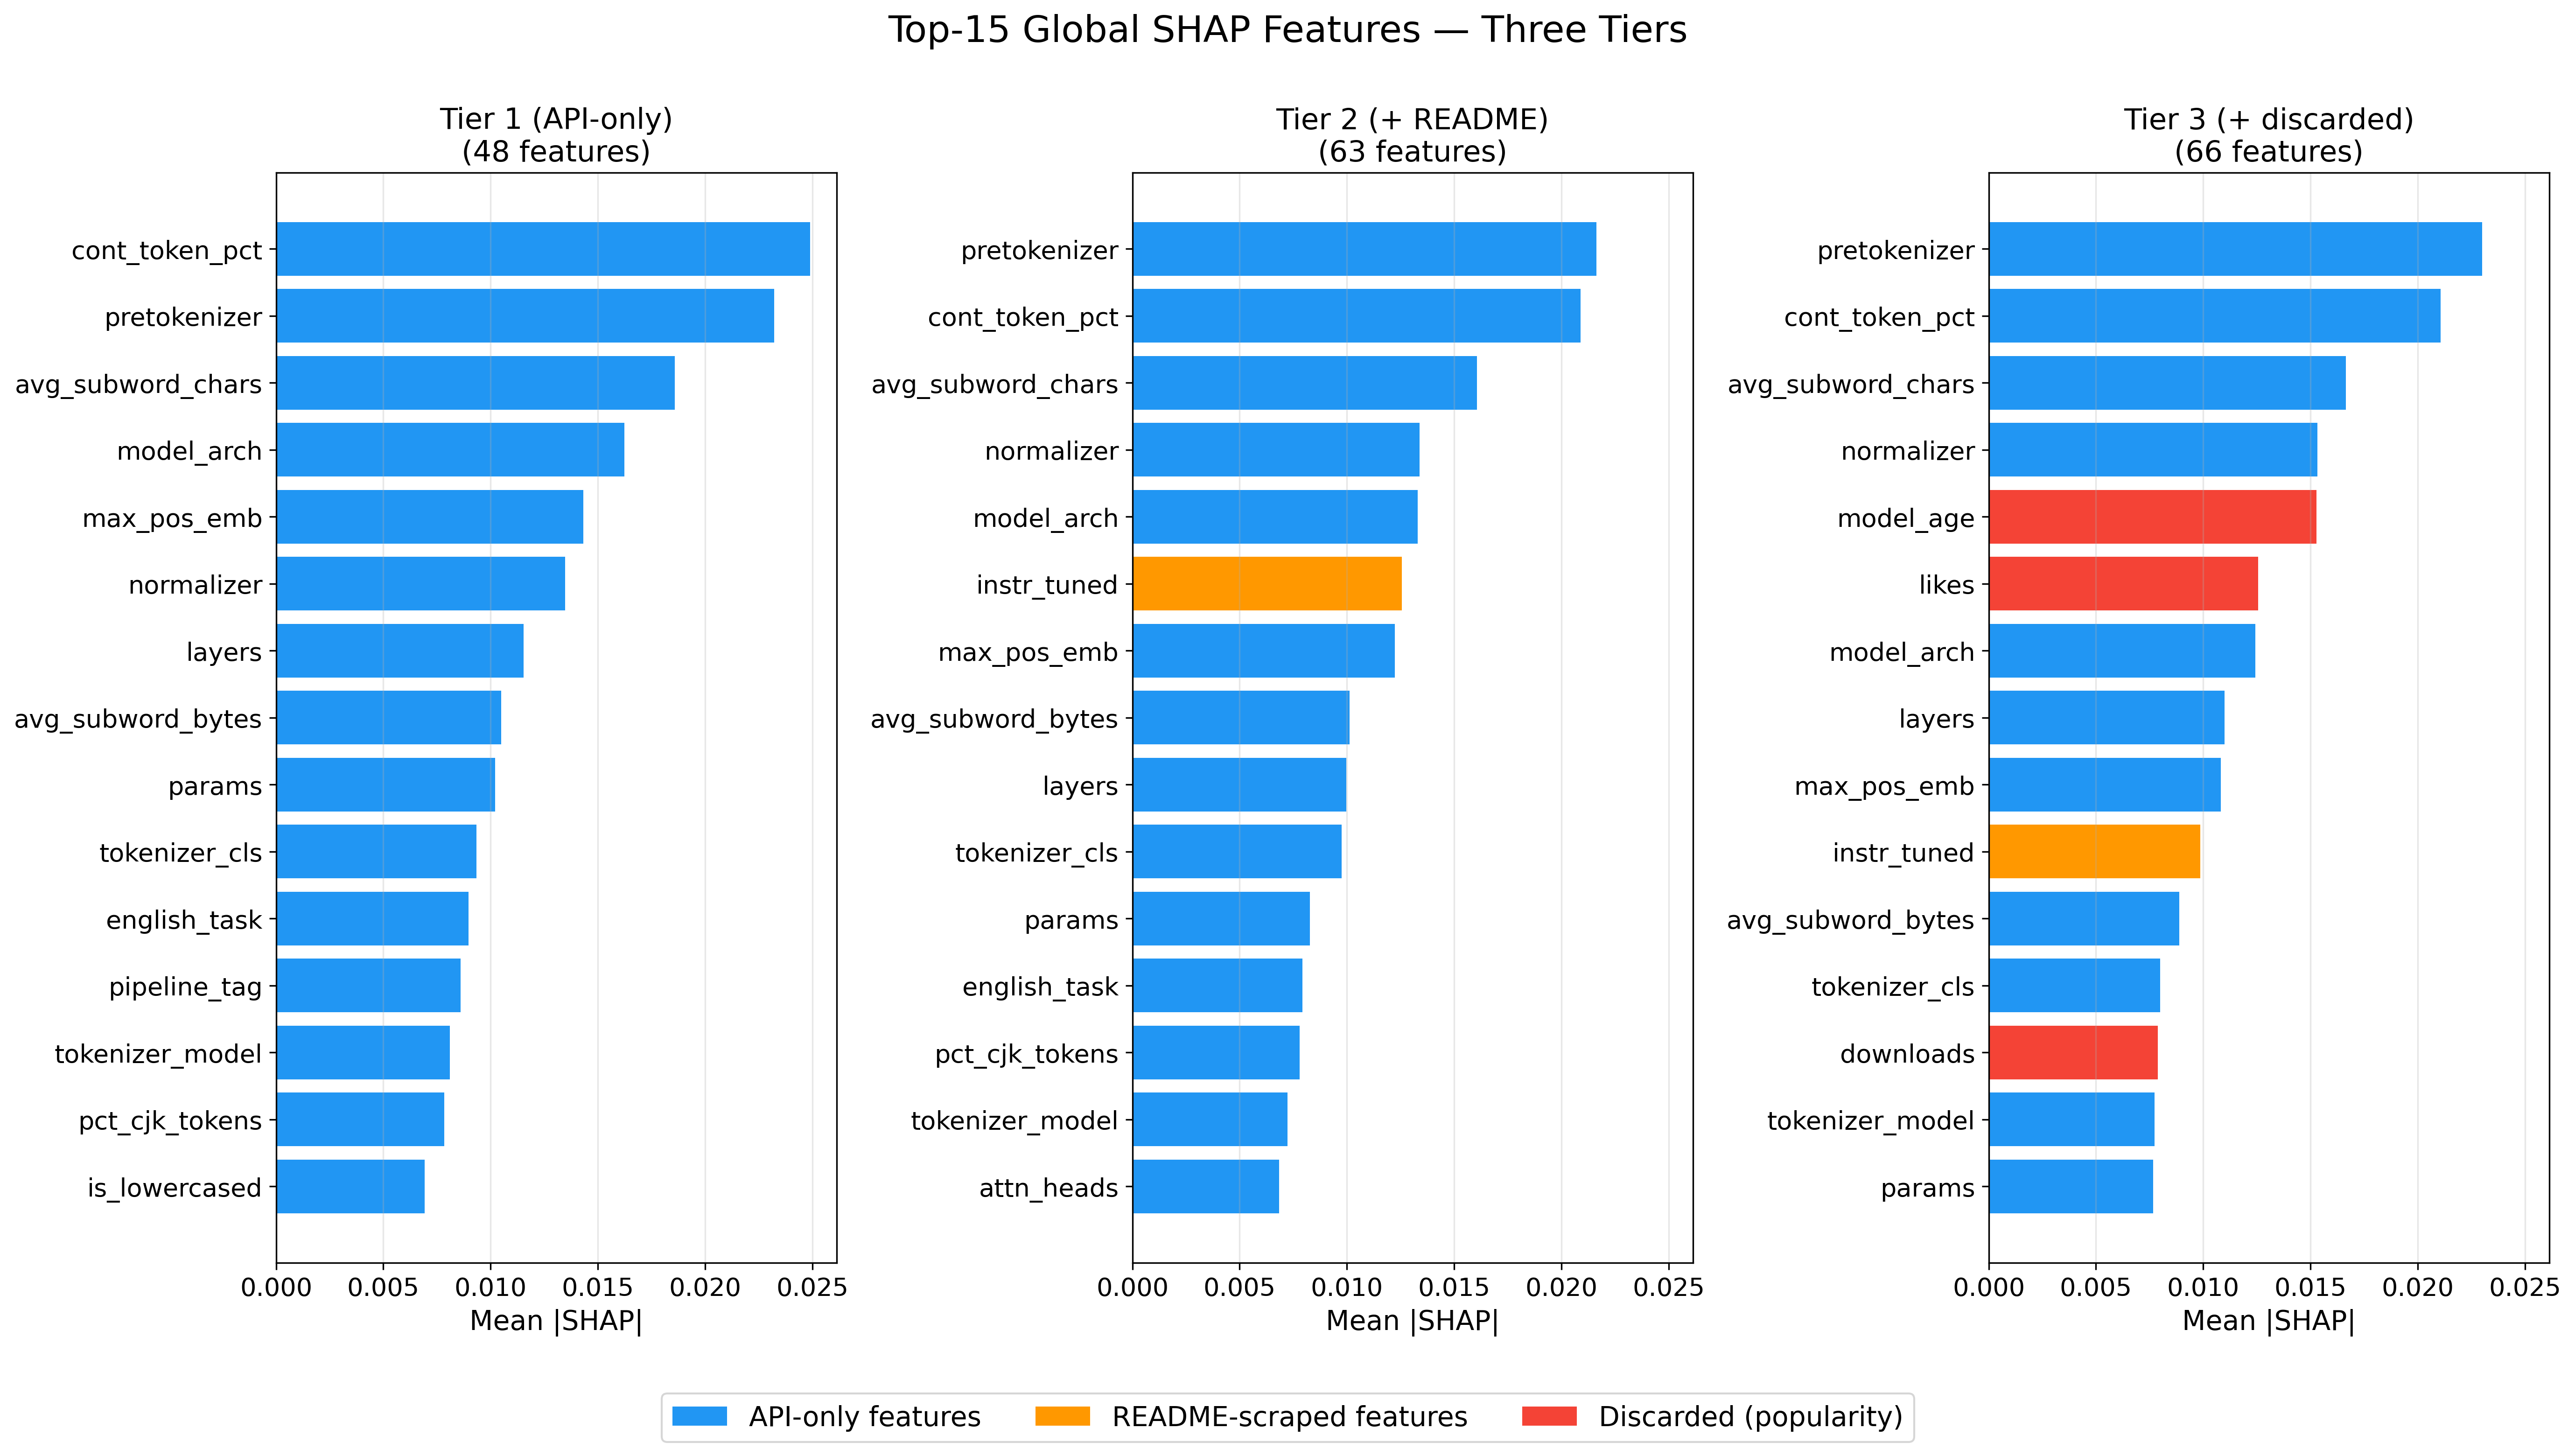
\includegraphics[width=\textwidth]{figures/shap_tier_comparison.png}
\caption{Top-15 global SHAP features for each tier (feature labels abbreviated for readability). Blue: API-only features; orange: README-scraped features; red: discarded popularity proxies.}
\label{fig:shap}
\end{figure*}

Across all three tiers, tokenizer-level features dominate the top of the ranking.
The percentage of continuation tokens---a measure of how much the tokenizer segments words into subword pieces---consistently ranks first or second, with a mean~$|\text{SHAP}|$ of 0.031 in Tier~2, roughly 50\% higher than the second-ranked feature.
\texttt{pretokenizer} (describing token processing steps such as byte-level encoding or whitespace splitting) ranks second, followed by average subword length.

It is important to note that these tokenizer features are not independent from each other or from the training data a model was exposed to.
A tokenizer trained on multilingual corpora, for instance, will naturally exhibit a higher percentage of continuation tokens and different script coverage than one trained on English-only data.
Similarly, \texttt{model\_arch} and \texttt{normalizer} both capture aspects of the overall model family (e.g.\ BERT-style vs.\ GPT-style), which is itself correlated with training methodology and data.
The high SHAP values for these features therefore reflect that they are informative \emph{proxies}---likely confounders rather than causal drivers---for the broader set of design and training choices that shape model quality (see Section~\ref{sec:discussion} for a more detailed discussion).

Among the README-scraped features, \texttt{instr\_tuned} is the most prominent (rank~7 in Tier~2), which aligns with the growing evidence that instruction tuning benefits embedding quality.
The training-data keyword flags (e.g.\ \texttt{train\_nli}, \texttt{train\_msmarco}) individually contribute modest SHAP values.
This likely understates the true importance of training data, since our keyword-matching approach can only approximate what data a model was actually trained on, and the real effect is distributed across many correlated flags.
Training data composition is almost certainly one of the most important factors in embedding model quality, but it is difficult to capture precisely from README text alone.

In Tier~3, the discarded features \texttt{model\_age} and \texttt{likes} enter the top-15 at ranks 4 and 7.
This is expected: newer and more popular models tend to incorporate the latest training techniques and larger datasets.
However, these are confounds rather than actionable features---a model does not become better by receiving more downloads.

\subsection{Feature Correlation and Redundancy}
\label{sec:correlation}

Several architecture features are highly correlated (Table~\ref{tab:correlations}).
In particular, \texttt{hidden\_dim}, \texttt{emb\_dim}, \texttt{ffn\_size}, and \texttt{attn\_heads} form a cluster with all pairwise Pearson~$|r| \geq 0.85$.
This is unsurprising: transformer architectures are typically scaled by increasing all of these dimensions jointly.

\begin{table*}[t]
\centering
\caption{Feature pairs with Pearson $|r| \geq 0.85$ in Tier~2.}
\label{tab:correlations}
\begin{tabular}{llc}
\toprule
Feature 1 & Feature 2 & $r$ \\
\midrule
hidden\_dim & emb\_dim & 0.974 \\
avg\_subword\_chars & median\_subword\_chars & 0.941 \\
hidden\_dim & ffn\_size & 0.897 \\
vocab\_size & actual\_vocab & 0.890 \\
ffn\_size & emb\_dim & 0.873 \\
attn\_heads & emb\_dim & 0.864 \\
\bottomrule
\end{tabular}
\end{table*}

Using connected-component analysis at a threshold of $|r| \geq 0.85$, we identify one cluster of four features: \texttt{hidden\_dim}, \texttt{attn\_heads}, \texttt{ffn\_size}, and \texttt{emb\_dim}.
We retain \texttt{hidden\_dim} as the representative (it has the largest ablation impact) and drop the other three, yielding a lean model of 66~features.
This lean model achieves an $R^2$ of 0.627---marginally \emph{better} than the 69-feature baseline (0.626), confirming that the dropped features were redundant.

\subsection{Ablation Study}

We perform a leave-one-feature-out ablation: for each of the 69~Tier~2 features, we remove it and re-evaluate the LOT-O~$R^2$.
Figure~\ref{fig:ablation} shows the $R^2$ change for each removed feature.

\begin{figure*}[t]
\centering
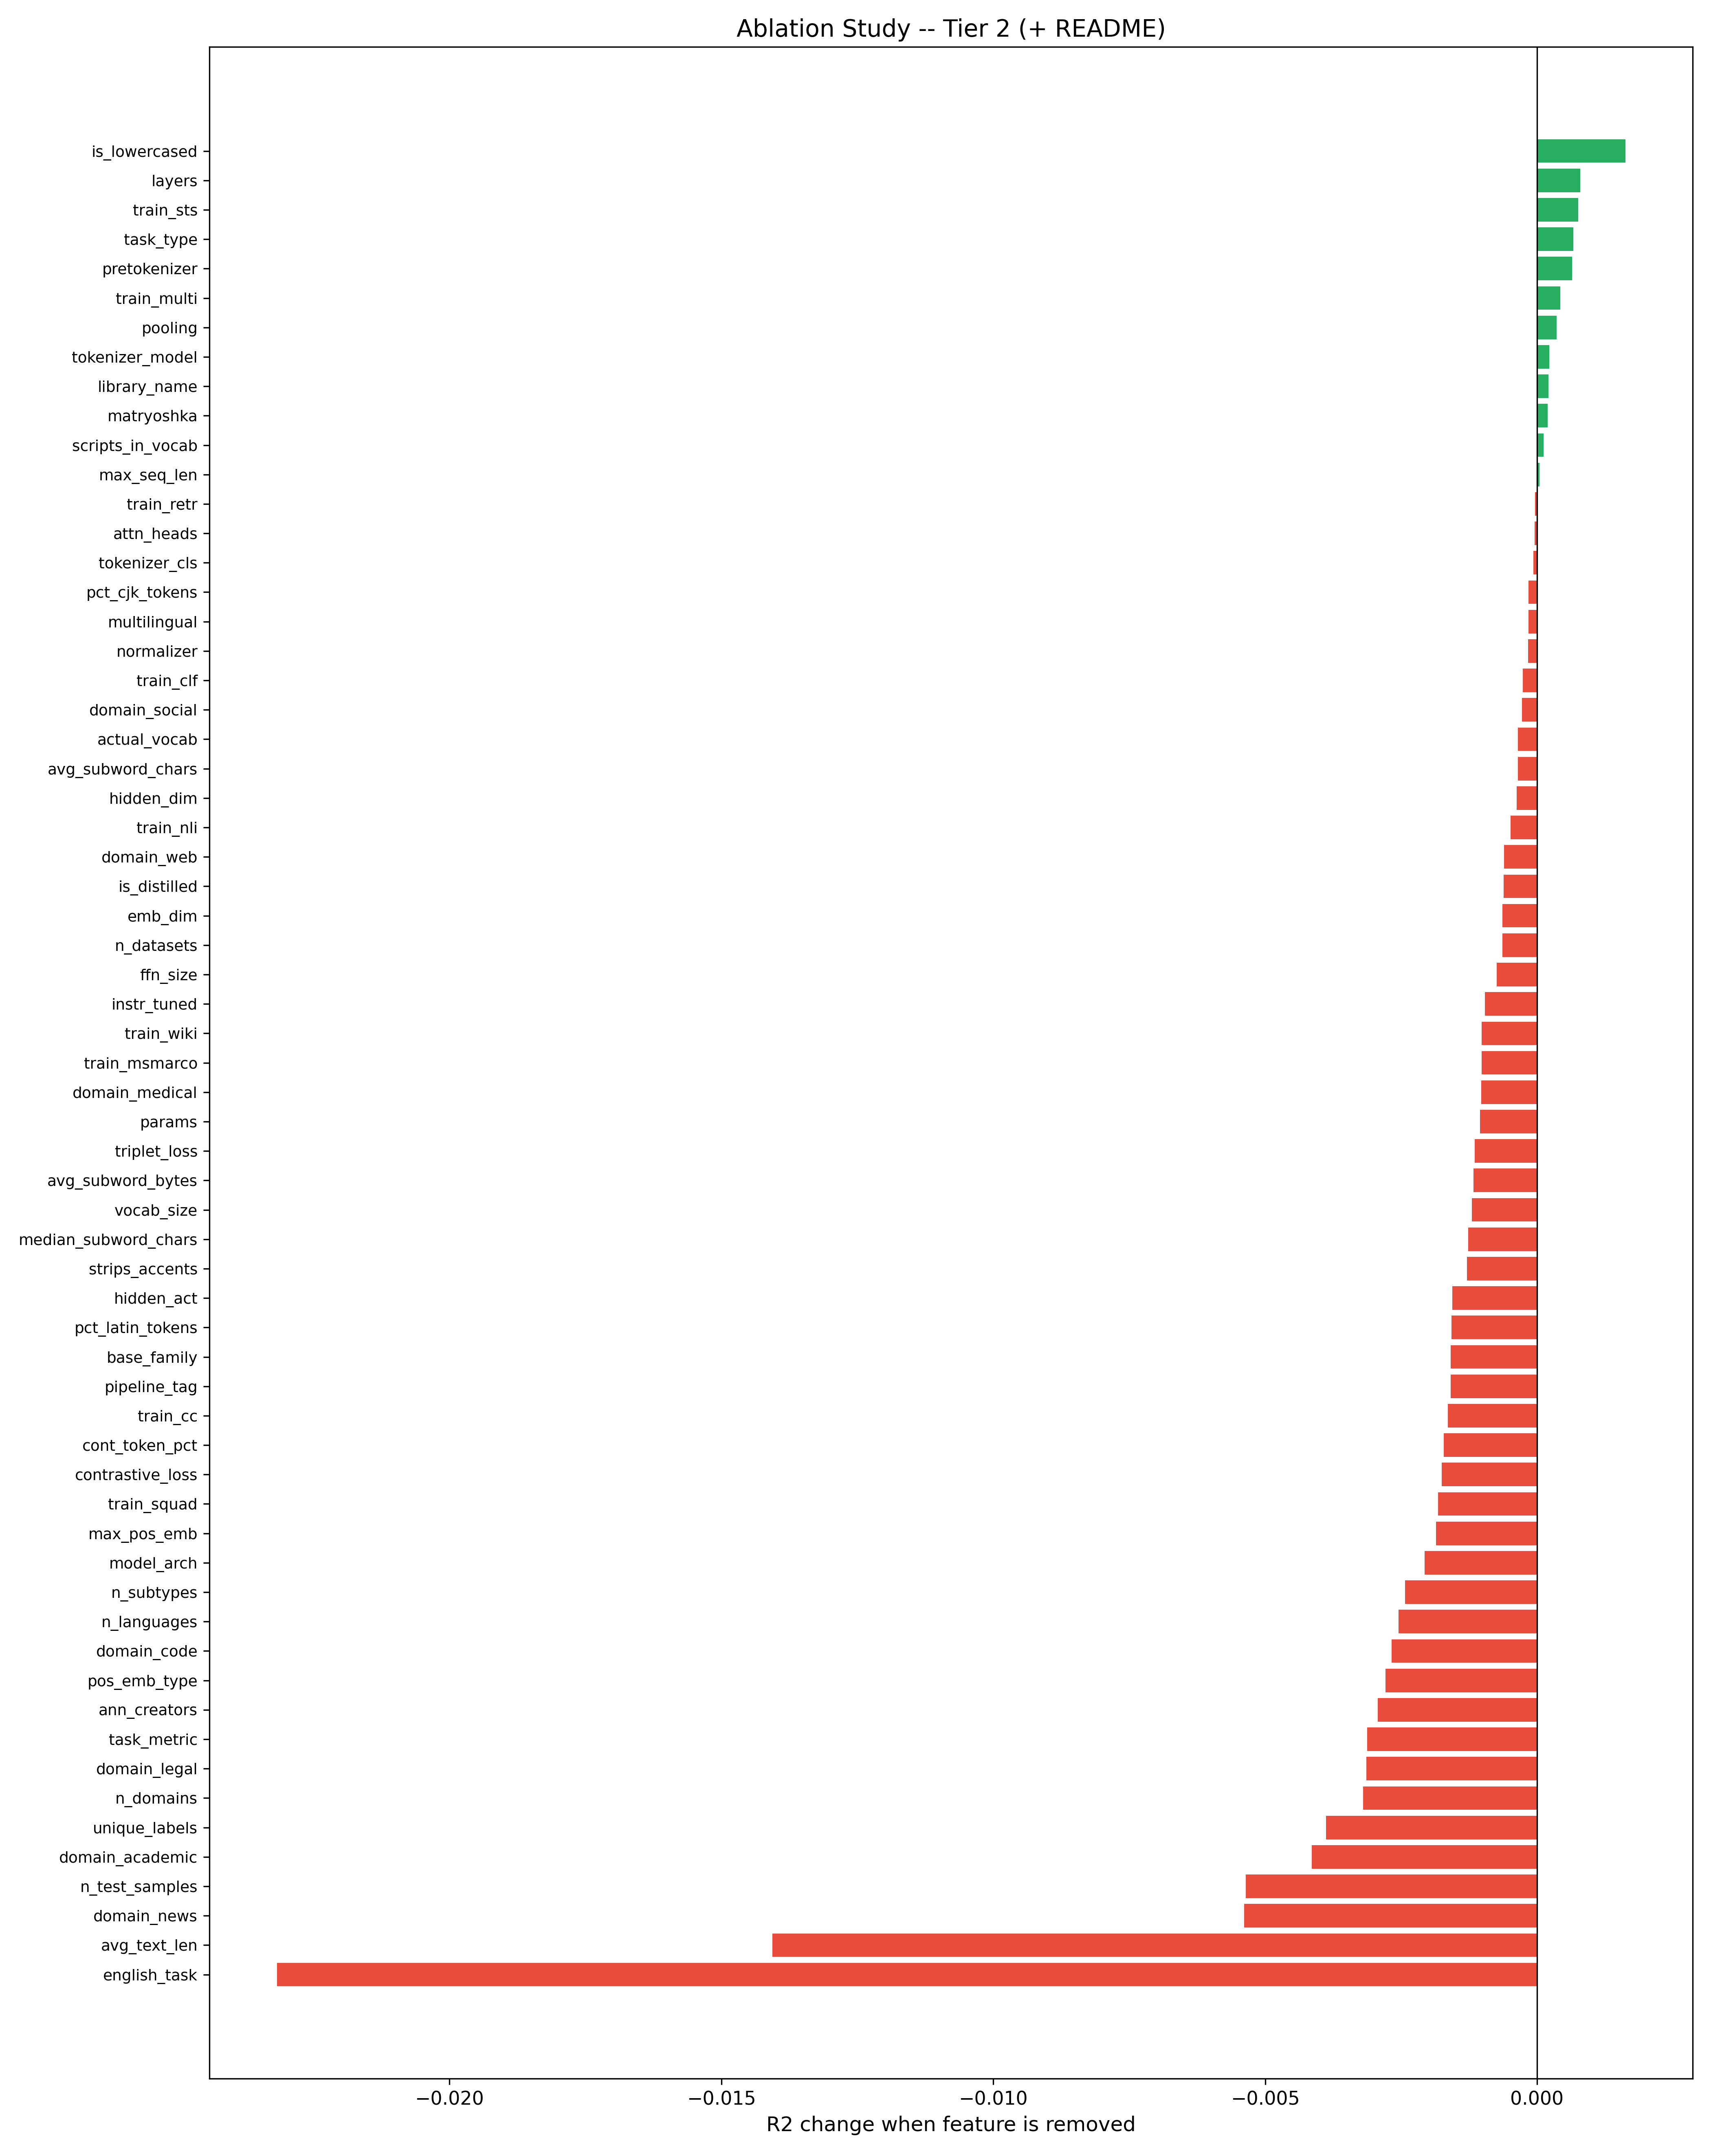
\includegraphics[height=0.86\textheight,keepaspectratio]{figures/ablation_study.png}
\caption{Change in LOT-O $R^2$ when each feature is removed from Tier~2 (feature labels abbreviated for readability).}
\label{fig:ablation}
\end{figure*}

The single most impactful feature is \texttt{english\_task}: removing it drops $R^2$ by 0.020.
This is a task-side feature indicating whether English is among the task's languages, and it acts as a broad partitioning variable---models and tasks behave very differently in multilingual versus English-only settings.
The next most impactful features are \texttt{avg\_text\_len} ($-$0.007), \texttt{ann\_creators} ($-$0.004), and \texttt{multilingual} ($-$0.004), all task-side descriptors.

On the model side, no single feature removal causes a large $R^2$ drop, which is consistent with the correlated-cluster structure observed in Section~\ref{sec:correlation}: when one architecture feature is removed, the correlated partners compensate.
This means the model's total knowledge about architecture size is resilient to losing any single feature, but it also makes it harder to attribute importance to individual features.

Several features can be removed with a marginal \emph{improvement} in $R^2$ (up to $+$0.002), suggesting mild overfitting or noise from those features.
Notably, \texttt{model\_arch} and \texttt{pos\_emb\_type}---both high-cardinality categoricals---show slight improvements when removed, possibly because label-encoding these features introduces arbitrary ordinal structure that the tree model occasionally overfits to.


% ══════════════════════════════════════════════════════════
\section{Discussion}
\label{sec:discussion}
% ══════════════════════════════════════════════════════════

\paragraph{Tokenizer features are surprisingly informative.}
The most striking finding of this study is the prominence of tokenizer-level features.
Rather than parameter count or layer depth, it is properties like the continuation-token ratio and \texttt{pretokenizer} that carry the most SHAP importance.
One plausible explanation is that these features serve as a fingerprint for the model's broader design lineage: a BPE tokenizer with a byte-level pre-tokenizer, for instance, is characteristic of modern GPT-style models, while a WordPiece tokenizer with a BERT normaliser signals the BERT family.
Different model families embody substantially different training methodologies, data mixes, and architectural innovations, and the tokenizer specification happens to be a compact summary of these choices.
It is therefore important not to interpret the high SHAP values as evidence that, say, changing the continuation-token percentage would directly improve a model.
Rather, the tokenizer is informative because it is correlated with many other aspects of the model's development.
To state this more explicitly: we hypothesise that features such as the continuation-token ratio are \emph{confounders}, not causes.
It is highly unlikely that altering a model's subword segmentation statistics in isolation would meaningfully change its benchmark scores; rather, these statistics happen to fingerprint the constellation of architecture, training data, and optimisation choices that \emph{does} drive quality.
The predictive power we observe is therefore best understood as evidence that tokenizer design co-varies with the factors that matter, not that it is itself among them.

\paragraph{Training data matters most---but is hardest to measure.}
Our README-scraping approach uses keyword matching to detect whether a model's card mentions specific training datasets (e.g.\ MS MARCO, NLI corpora, Wikipedia).
While these flags do add predictive value (Tier~2 improves over Tier~1 by $+0.016$ in $R^2$), their individual SHAP values are modest.
We believe this understates the true importance of training data.
The fundamental limitation is that model cards vary enormously in detail and accuracy: some list every dataset; others describe the training data in vague terms or not at all.
Our binary keyword flags are therefore noisy proxies.
If one could obtain precise training data composition---corpus sizes, domain distributions, language mixes---these features would very likely dominate the importance rankings.
This remains one of the most important missing pieces in the current model metadata ecosystem.

\paragraph{Popularity proxies are confounded, not causal.}
Downloads, likes, and model age enter the Tier~3 top-15 SHAP features, but they do not meaningfully improve $R^2$ ($+0.004$).
These metrics are correlated with model quality because better models attract more usage, but they have no causal relationship with performance.
Their inclusion in Tier~3 serves as a sanity check: the fact that they provide minimal additional signal suggests that the Tier~2 features already capture the substantive variation.

\paragraph{Task-family heterogeneity.}
Retrieval and BitextMining tasks are most predictable ($R^2 > 0.7$), while Classification is hardest ($R^2 \approx 0.24$).
Classification tasks span a wide range of domains, label counts, and text lengths, making it harder for a single set of model features to predict performance across all of them.
This suggests that classification may benefit from task-specific feature engineering or a hierarchical modelling approach.

\paragraph{Non-linear models are essential.}
The gap between Ridge ($R^2 = 0.34$) and Random Forest ($R^2 = 0.63$) highlights the importance of non-linear interactions.
Features like \texttt{pretokenizer} or \texttt{model\_arch} interact with architecture size and task characteristics in ways that linear models cannot capture.
This is consistent with the intuition that a feature's effect on performance depends on the context: for example, a large model with a specific tokenizer type may behave very differently from a small model with the same tokenizer.


% ══════════════════════════════════════════════════════════
\section{Limitations}
\label{sec:limitations}
% ══════════════════════════════════════════════════════════

Several limitations should be considered when interpreting these results.

\paragraph{Training data opacity.}
As discussed, our README-based training data features are noisy approximations.
If we could add one feature that is currently unavailable for most models, it would be a \emph{detailed training data manifest}: the exact datasets used, their sizes, and the mixing proportions.
Training data composition is almost certainly the single largest driver of embedding model performance, and the inability to measure it precisely is the most important limitation of metadata-based prediction.

\paragraph{Confounding across features.}
Many of our features are mutually correlated---not only the architecture-size cluster, but also model family, tokenizer type, and training methodology.
SHAP values attribute importance to individual features but cannot fully disentangle causal contributions when features move together.
A model's ``base family'' (e.g.\ BERT vs.\ LLaMA) bundles together architecture, tokenizer, training data, and often training procedure, making it difficult to isolate the effect of any single factor.

\paragraph{Label encoding of categoricals.}
We use label encoding for categorical features such as \texttt{model\_arch} and \texttt{tokenizer\_cls}.
This imposes an arbitrary ordering that tree-based models can exploit but does not reflect a meaningful relationship. Although Random Forests are relatively robust to this, they may introduce noise, as suggested by the ablation result where removing \texttt{model\_arch} slightly improves $R^2$.
Target encoding or native categorical support (as in LightGBM) could be explored in future work.

\paragraph{Snapshot nature.}
Our data reflect the MTEB leaderboard at a single point in time.
As new models are released, the landscape may shift---particularly if new architectures or training techniques emerge that are not well represented in our feature set.

\paragraph{English-centric evaluation.}
Although MTEB includes multilingual tasks, the models in our sample are predominantly English or multilingual-with-English models.
Our results may not generalize to purely non-English settings.

\paragraph{Missing features.}
Beyond training data, several other features could be informative but are not available for most models: training hyperparameters (learning rate, batch size, number of steps), hardware used, fine-tuning details, and quantitative measures of data quality.
A feature that captures the \emph{diversity} or \emph{difficulty} of the training data would be particularly valuable.


% ══════════════════════════════════════════════════════════
\section{Conclusion}
\label{sec:conclusion}
% ══════════════════════════════════════════════════════════

We have shown that a substantial fraction of the performance variation among text embedding models on the MTEB benchmark can be predicted from publicly available metadata.
A Random Forest trained on 69~features achieves a mean leave-one-task-out~$R^2$ of~0.63, with Retrieval and BitextMining tasks being most predictable and Classification least.
Tokenizer-level features---in particular the continuation-token ratio and \texttt{pretokenizer}---emerge as the strongest individual predictors, serving as compact proxies for the model's broader design lineage.
README-scraped training-data flags add modest predictive value ($+0.016$ in $R^2$), while popularity metrics contribute negligibly.
A correlation-based redundancy analysis reduces the feature set from 69~to 66~features with no loss in performance.

These results suggest that the metadata accompanying models on public hubs carries meaningful signal about quality, and that enriching this metadata---particularly with standardised training data documentation---could enable better model selection without exhaustive evaluation.
For practitioners, our analysis highlights that looking beyond parameter count to tokenizer properties and training methodology can be more informative when assessing embedding models.

\newpage

% ══════════════════════════════════════════════════════════
% References
% ══════════════════════════════════════════════════════════

\begin{thebibliography}{9}

\bibitem[Xia et~al.(2020)]{xia2020predicting}
Mengzhou Xia, Antonios Anastasopoulos, Ruochen Xu, Yiming Yang, and Graham Neubig.
\newblock Predicting performance for natural language processing tasks.
\newblock In \emph{Proceedings of the 58th Annual Meeting of the Association for Computational Linguistics}, pages 8625--8646, 2020.

\bibitem[Owen(2024)]{owen2024predictable}
David Owen.
\newblock How predictable is language model benchmark performance?
\newblock \emph{arXiv preprint arXiv:2401.04757}, 2024.

\bibitem[Muennighoff et~al.(2023)]{muennighoff2023mteb}
Niklas Muennighoff, Nouamane Tazi, Lo\"ic Barrault, and Douwe Kiela.
\newblock {MTEB}: Massive Text Embedding Benchmark.
\newblock In \emph{Proceedings of the 17th Conference of the European Chapter of the Association for Computational Linguistics}, pages 2014--2037, 2023.

\bibitem[Lundberg \& Lee(2017)]{lundberg2017shap}
Scott~M. Lundberg and Su-In Lee.
\newblock A unified approach to interpreting model predictions.
\newblock In \emph{Advances in Neural Information Processing Systems}, volume~30, 2017.

\bibitem[Kaplan et~al.(2020)]{kaplan2020scaling}
Jared Kaplan, Sam McCandlish, Tom Henighan, Tom~B. Brown, Benjamin Chess, Rewon Child, Scott Gray, Alec Radford, Jeffrey Wu, and Dario Amodei.
\newblock Scaling laws for neural language models.
\newblock \emph{arXiv preprint arXiv:2001.08361}, 2020.

\bibitem[Hoffmann et~al.(2022)]{hoffmann2022training}
Jordan Hoffmann, Sebastian Borgeaud, Arthur Mensch, Elena Buchatskaya, Trevor Cai, Eliza Rutherford, Diego de~Las~Casas, Lisa~Anne Hendricks, Johannes Welbl, Aidan Clark, Tom Hennigan, Eric Noland, Katie Millican, George van~den~Driessche, Bogdan Damoc, Aurelia Guy, Simon Osindero, Karen Simonyan, Erich Elsen, Jack~W.\ Rae, Oriol Vinyals, and Laurent Sifre.
\newblock Training compute-optimal large language models.
\newblock In \emph{Advances in Neural Information Processing Systems}, volume~35, 2022.

\end{thebibliography}

\newpage

% ══════════════════════════════════════════════════════════
% Appendix
% ══════════════════════════════════════════════════════════

\appendix
\section{Figures}
\label{app:figures}

\begin{figure*}[H]
\centering
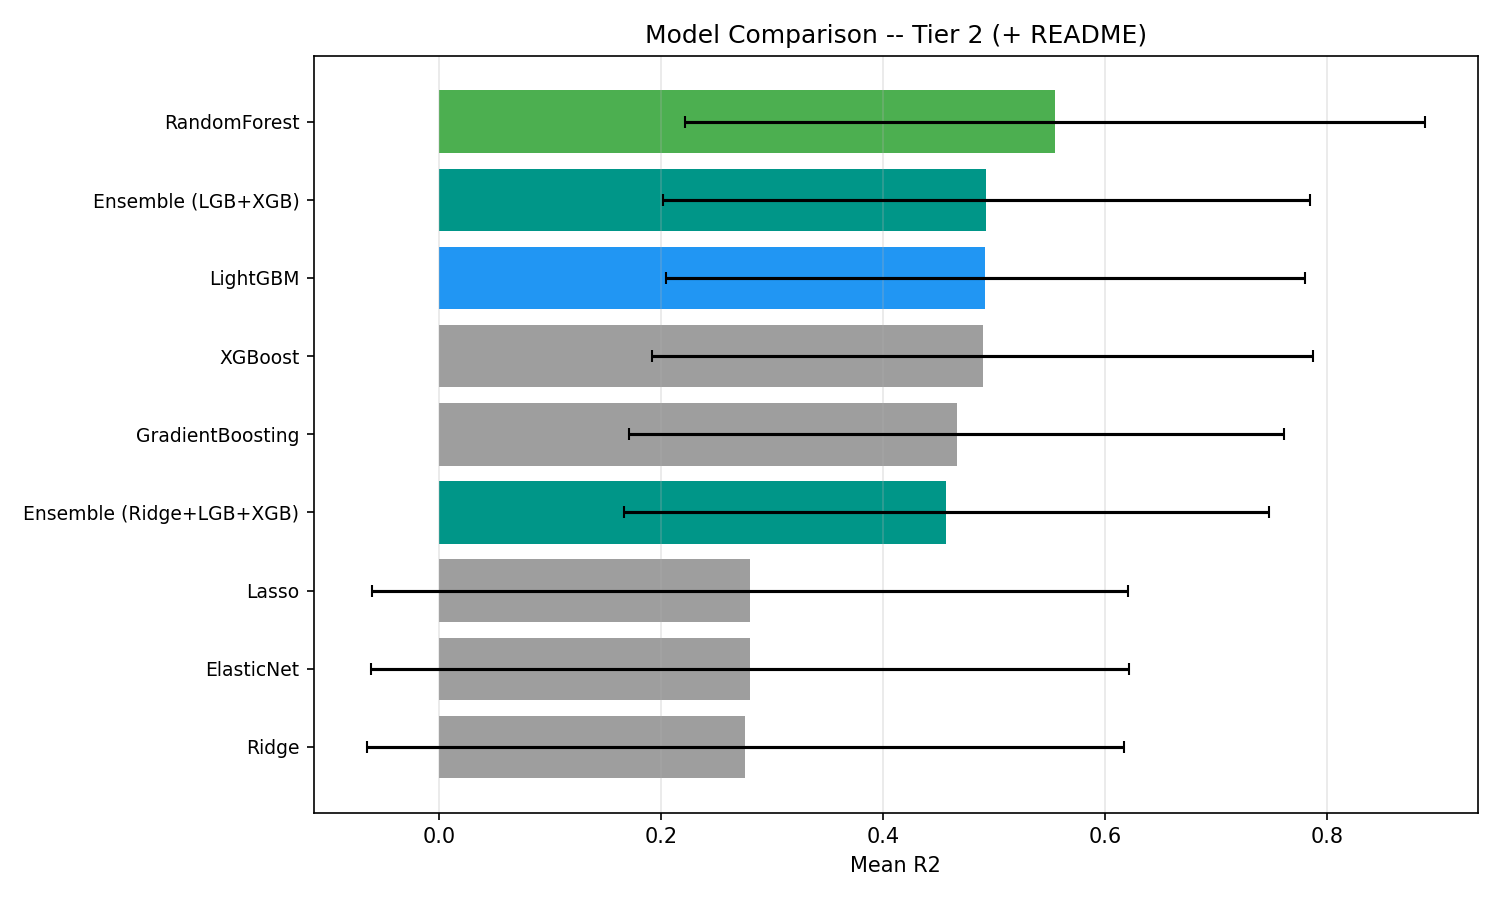
\includegraphics[width=0.9\textwidth]{figures/model_comparison.png}
\caption{Model comparison bar chart (Tier~2 features).}
\label{fig:model_comparison}
\end{figure*}

\begin{figure*}[H]
\centering
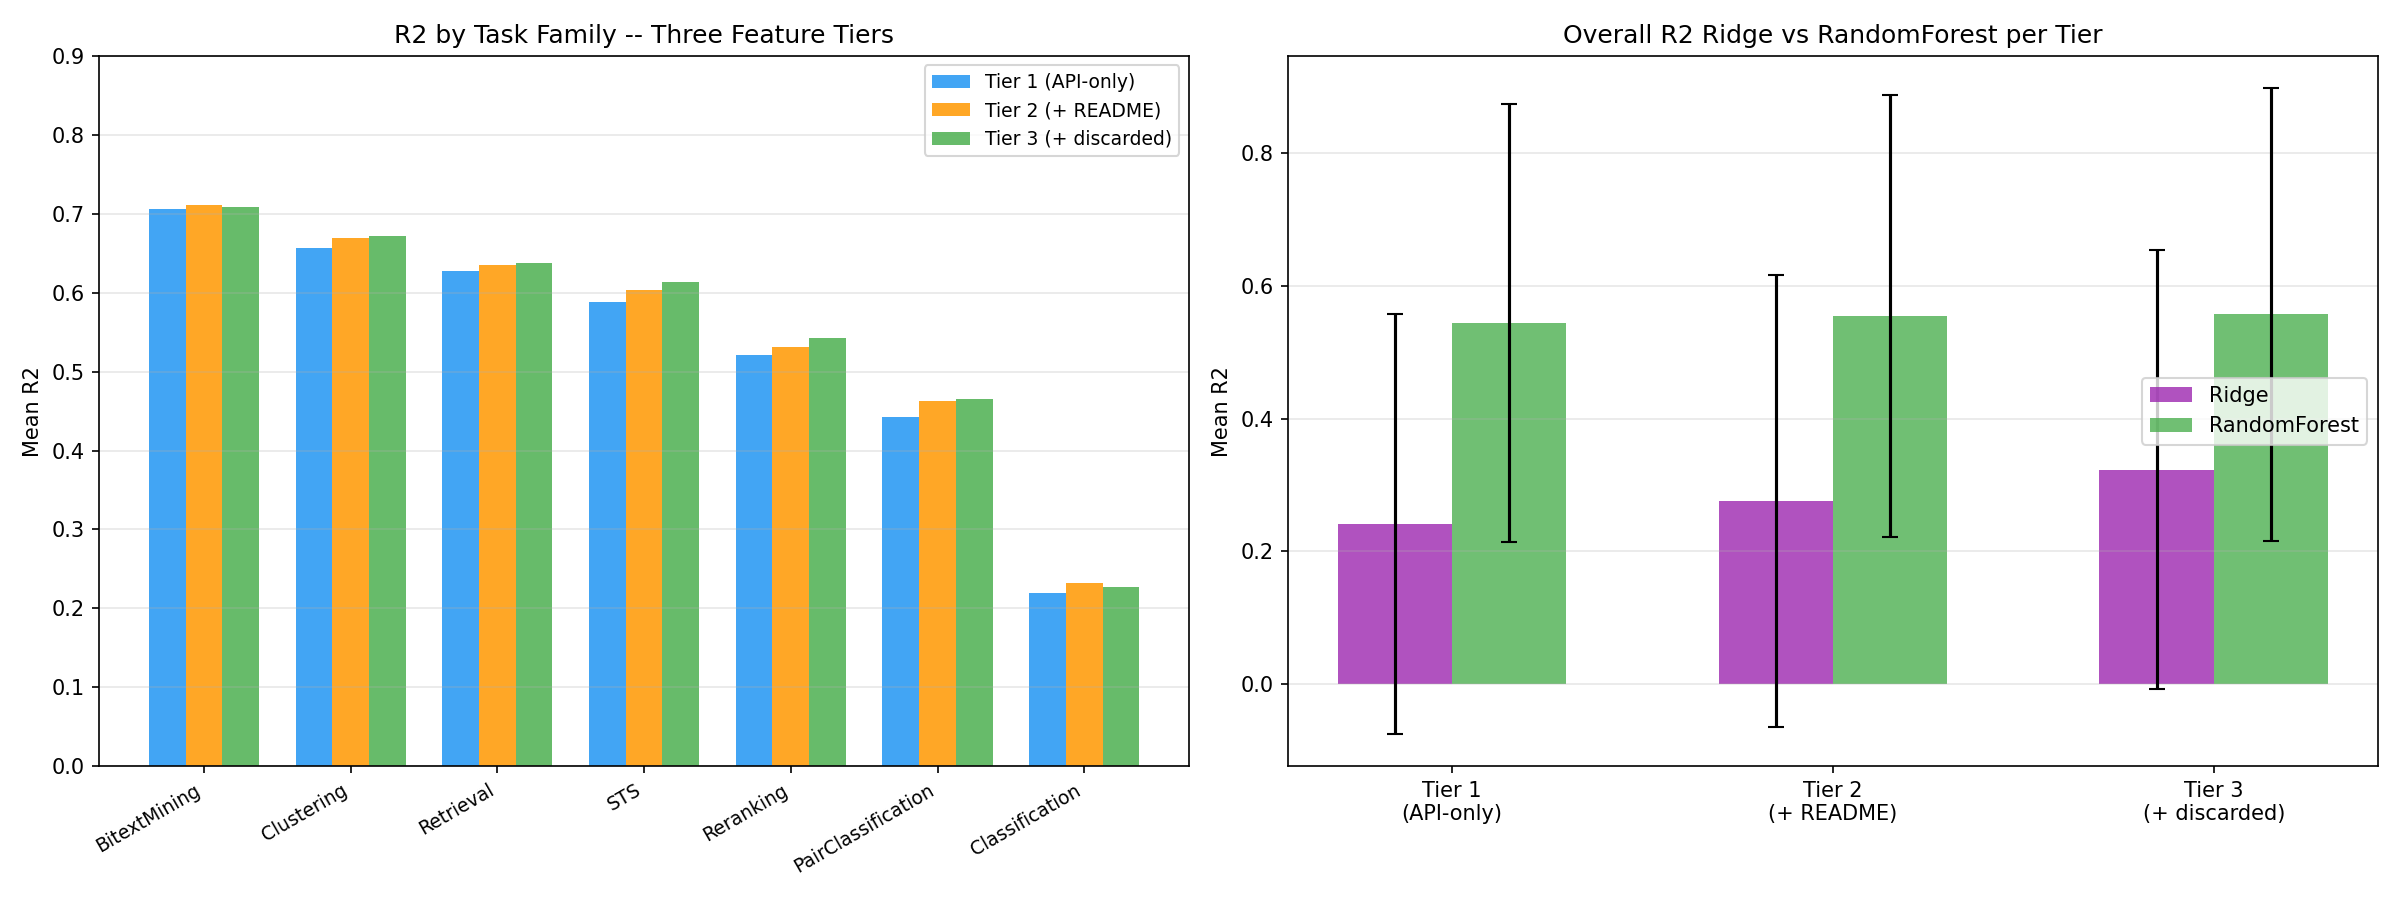
\includegraphics[width=\textwidth]{figures/tier_comparison.png}
\caption{Tier comparison: (left) per-family $R^2$ across tiers; (right) overall Ridge vs.\ RF $R^2$ per tier.}
\label{fig:tier_comparison}
\end{figure*}

\end{document}
